\begin{figure}[H]
	\begin{minipage}[t]{0.45\linewidth}
	\centering
	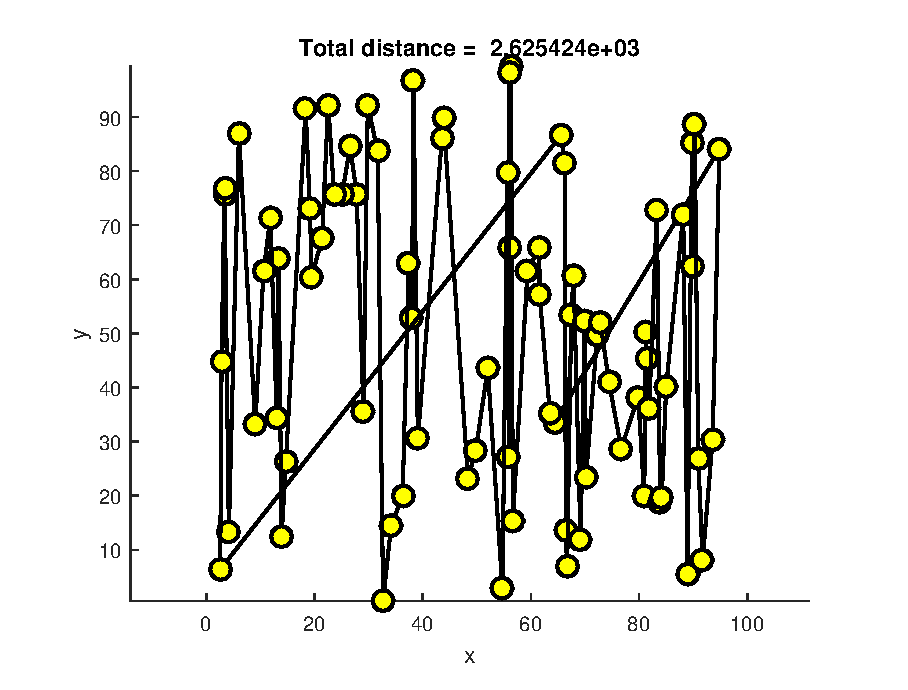
\includegraphics[width=\textwidth]{\Pathofcent/path.eps}
	\caption{Path journey}\label{fig:Pathofcent:path}
	
	\end{minipage}\hfill
	\begin{minipage}[t]{0.45\linewidth}
	\centering
	\includegraphics[width=\textwidth]{\Pathofcent/AS_1_5AS_ExecTimeAndMeanSTDWith_execVariation.eps}
	\caption{Variation of the execution time VS the \# of ants (20$\stackrel{step=20}{\rightarrow}$100) in each execution (1$\stackrel{step=1}{\rightarrow}$ 5)}
	\label{fig:Pathofcent:AS_1_5AS_ExecTimeAndMeanSTDWith_execVariation}
	\end{minipage}
	\flushleft
	\begin{minipage}[t]{0.45\linewidth}
	\centering
	\includegraphics[width=1.5\textwidth,height=.9\textwidth]{\Pathofcent/AS_BestCost_Varying_Iteration_and_nbAnts.eps}
	\caption{Best cost VS Ants number variation with $\alpha$=1, $ \beta $ = 5}
	\label{fig:Pathofcent:AS_BestCost_Varying_Iteration_and_nbAnts}
	\end{minipage}
%%	\vspace{length}
\end{figure}
	\begin{minipage}[t]{0.9\linewidth}
	\vspace{-9mm}
	\begin{table}[H]
	\label{tab:Pathofcent:expdeux}
	\begin{tabular}{lllll}
	\cline{1-2}
	\multicolumn{1}{|l|}{Best Costs results for experience 2 on rand100.dat }                                                           &  \multicolumn{1}{l|}{Elapsed Time, Mean, STD}                                             &  &  &  \\ \cline{1-2}
	\multicolumn{1}{|l|}{\begin{tiny}\begin{tabular}{|l|c|c|c|c|c|c|c|c|c|c|}
\hline
&\textbf{It :1}&\textbf{It :2}&\textbf{It :3}&\textbf{It :4}&\textbf{It :5}&\textbf{It :6}&\textbf{It :7}&\textbf{It :8}&\textbf{It :9}&\textbf{It :10}\\\hline
\textbf{exec :1}&1075.02&1075.02&989.30&989.30&989.30&989.30&989.30&989.30&989.30&989.30\\\hline
\textbf{exec :2}&1070.27&1001.81&1001.81&1001.81&1001.81&1001.81&1001.81&1001.81&1001.81&1001.81\\\hline
\textbf{exec :3}&1086.19&1068.87&1040.86&1040.86&1040.86&1020.56&1020.56&1004.34&1004.34&1004.34\\\hline
\textbf{exec :4}&1102.86&1063.08&1063.08&1030.00&1016.38&1016.38&1016.38&1016.38&1016.38&977.46\\\hline
\textbf{exec :5}&1044.44&1044.44&1044.44&1044.44&1044.44&1044.44&1044.44&1044.44&1015.33&1015.33\\\hline
\textbf{exec :6}&1062.82&1062.82&1028.11&1028.11&1028.11&1028.11&1028.11&1028.11&1028.11&1028.11\\\hline
\textbf{exec :7}&1063.06&1020.15&1020.15&1020.15&1020.15&1020.15&1020.15&1020.15&1020.15&1020.15\\\hline
\textbf{exec :8}&1054.73&1052.78&1052.78&999.26&999.26&999.26&993.55&993.55&993.55&993.55\\\hline
\textbf{exec :9}&1078.24&1041.31&1041.31&1041.31&1041.31&1041.31&1041.31&1041.31&1041.31&1041.31\\\hline
\textbf{exec :10}&967.51&967.51&967.51&967.51&967.51&967.51&967.51&967.51&967.51&967.51\\\hline
\end{tabular}
\end{tiny}} & \multicolumn{1}{l|}{\begin{tiny}\begin{tabular}{|l|c|}
\hline
&\textbf{Elapsed time}\\\hline
\textbf{exec :1}&2.63\\\hline
\textbf{exec :2}&4.37\\\hline
\textbf{exec :3}&6.15\\\hline
\textbf{exec :4}&7.89\\\hline
\textbf{exec :5}&9.85\\\hline
\textbf{exec :6}&18.70\\\hline
\textbf{exec :7}&27.65\\\hline
\textbf{exec :8}&36.37\\\hline
\textbf{exec :9}&44.87\\\hline
\textbf{exec :10}&89.32\\\hline
\textbf{ Mean}&24.78\\\hline
\textbf{ STD}&26.90\\\hline
\end{tabular}
\end{tiny} } &  &  &  \\ \cline{1-2}
	&     &  &  &  \\
	&     &  &  & 
	\end{tabular}
	\caption{Results of experience 2 on rand100.dat}
	\end{table}
	\end{minipage}